\documentclass[border=10pt]{standalone}

\usepackage{tikz}
\usetikzlibrary{shapes,arrows}

\begin{document}


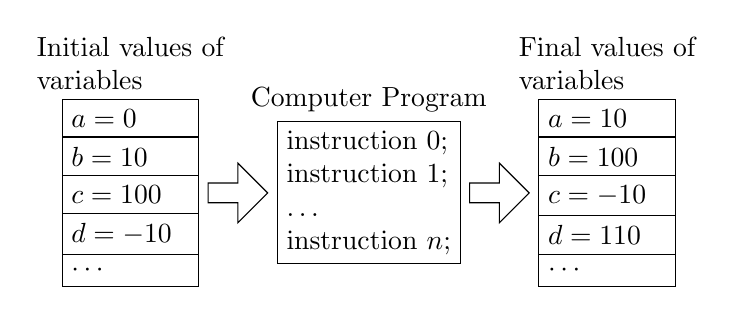
\begin{tikzpicture}[every text node part/.style={align=left},
                     stack/.style={rectangle split, 
                                   rectangle split parts = 5, 
                                   draw,text width=1.5cm},
                    myarrow/.style={single arrow,
                                    draw,
                                    right = 3pt,
                                    minimum size = 5ex}
                  ]
% we start
\node [stack] (ini)  {%
                      $a=0$     \nodepart{two}
                      $b=10$    \nodepart{three}
                      $c=100$   \nodepart{four}
                      $d=-10$   \nodepart{five}
                      $\cdots$};
% we add an arrow
\node [myarrow] (A) at (ini.east) {} ;  
% after the arrow, the main node at the end
\node [draw,rectangle,align=left,right=3pt] (mid) at (A.east)
            {instruction 0;\\ 
             instruction 1;\\
             $\ldots$\\
             instruction $n$;};
% we add another arrow
\node [myarrow] (B) at (mid.east) {} ;   
% after the arrow, the final node 
\node [stack,right=3pt] (fin) at (B.east)  {%
                                            $a=10$    \nodepart{two}
                                            $b=100$   \nodepart{three}
                                            $c=-10$   \nodepart{four}
                                            $d=110$   \nodepart{five}
                                            $\cdots$};
% labels : I don't like vey much `label= ` it's a shortcut but I think it's more powerful and flexible to use real nodes.
\node [above,align=left]  at (ini.north) {Initial values of\\
                                          variables};
\node [above,align=left]  at (fin.north) {Final values of\\
                                          variables};
\node [above]             at (mid.north) {Computer Program};   

\end{tikzpicture}
\end{document}
